\begin{Schunk}
\begin{Sinput}
> library("Ham94", lib.loc = "../../../library")
\end{Sinput}
\end{Schunk}
Example 4.1 from page 112 illustrates the Box-Jenkins
approach based on autocorrelations.  Here the data series is log changes
of seasonally adjusted real US GNP from 1947 to 1988,
available by simple transformations of the data in object "gnp1996".
The data is prepared by selecting quarterly date from as shown, then computing the log of differences.
\begin{Schunk}
\begin{Sinput}
> data(gnp1996, package = "Ham94")
> selection <- subset(gnp1996, Quarter >= "1947-01-01" & Quarter <= 
+     "1988-10-01")
> y <- diff(log(selection$GNPH))
\end{Sinput}
\end{Schunk}
Page 110 shows how to compute sample autocorrelations - we will generate the first 20 to be used in plotting the results below.
\begin{Schunk}
\begin{Sinput}
> max.lags <- 20
> T <- length(y)
> threshold <- 2/sqrt(T)
> gammas <- vector(mode = "numeric", length = max.lags + 1)
> gammas[[1]] <- 1/T * t(y - mean(y)) %*% (y - mean(y))
> for (j in 1:max.lags) gammas[j + 1] <- 1/T * t((y - mean(y))[(j + 
+     1):T]) %*% (y - mean(y))[1:(T - j)]
> rhos <- gammas/gammas[[1]]
\end{Sinput}
\end{Schunk}
Page 111 shows how to compute sample partial autocorrelations.  
\begin{Schunk}
\begin{Sinput}
> subscripts <- outer(seq(1, max.lags), seq(1, max.lags), function(i, 
+     j) {
+     abs(i - j)
+ })
> GAMMA <- array(gammas[as.vector(subscripts) + 1], c(max.lags, 
+     max.lags))
> alphas <- vector(mode = "numeric", length = max.lags)
> for (m in 1:max.lags) alphas[m] <- solve(GAMMA[1:m, 1:m], gammas[2:(m + 
+     1)])[[m]]
\end{Sinput}
\end{Schunk}
A plot of the outputs reproducing figure 4.2 is shown below.  The source code is provided in the demo.
\begin{center}
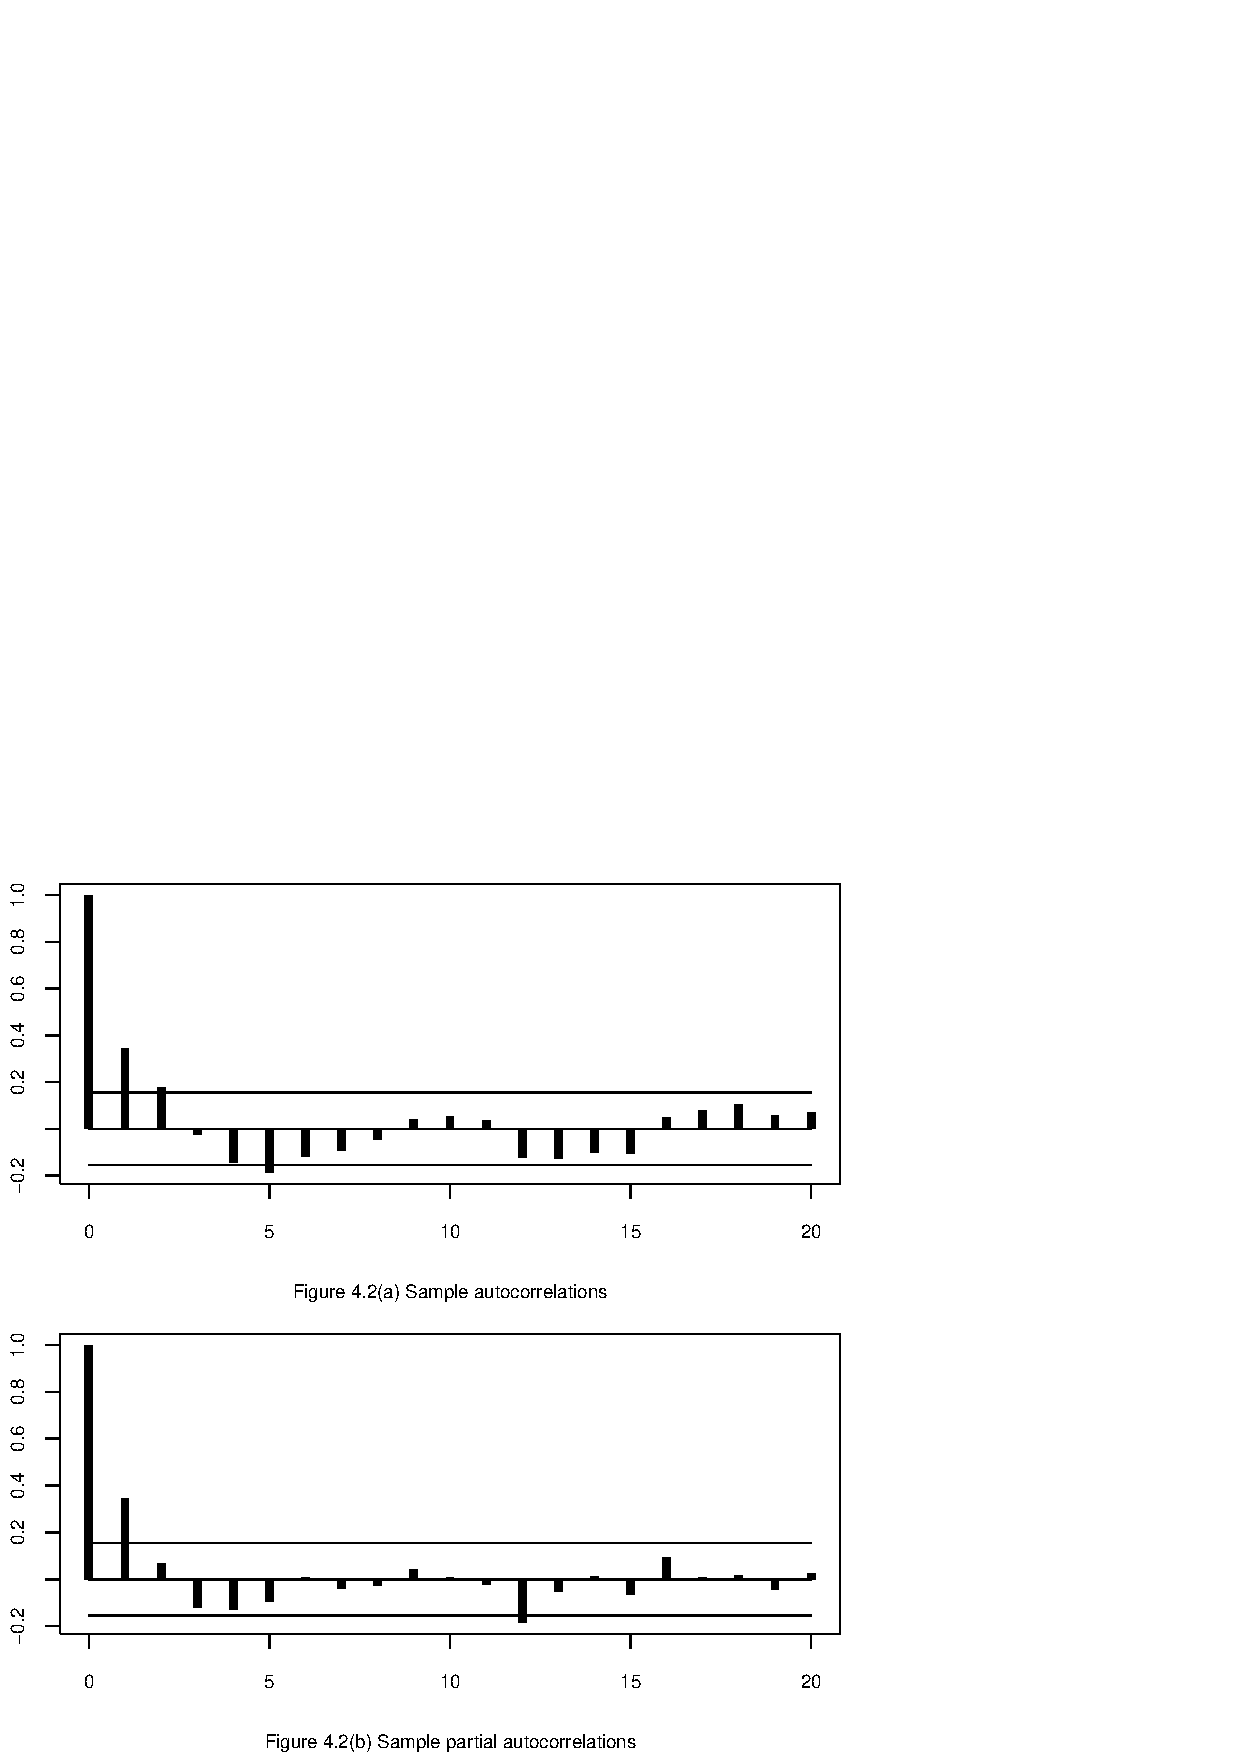
\includegraphics{p112-005}
\end{center}
\subsection{R Facilities for Sample Autocorrelations}
Function acf from R package "stats" performs the same function as acf, as we can readily
confirm.
\begin{Schunk}
\begin{Sinput}
> acf.correlation <- acf(y, lag.max = max.lags, type = "correlation", 
+     plot = FALSE, demean = TRUE)
> print(as.vector(acf.correlation$acf))
\end{Sinput}
\begin{Soutput}
 [1]  1.00000000  0.34509475  0.17817758 -0.02537843 -0.14230681 -0.18827409
 [7] -0.11613672 -0.09335581 -0.04441490  0.03902657  0.05412612  0.03788102
[13] -0.12386994 -0.12725888 -0.10256196 -0.10719806  0.05022865  0.07874423
[19]  0.10451845  0.05540046  0.07001701
\end{Soutput}
\begin{Sinput}
> print(rhos)
\end{Sinput}
\begin{Soutput}
 [1]  1.00000000  0.34509475  0.17817758 -0.02537843 -0.14230681 -0.18827409
 [7] -0.11613672 -0.09335581 -0.04441490  0.03902657  0.05412612  0.03788102
[13] -0.12386994 -0.12725888 -0.10256196 -0.10719806  0.05022865  0.07874423
[19]  0.10451845  0.05540046  0.07001701
\end{Soutput}
\begin{Sinput}
> acf.partial <- acf(y, lag.max = max.lags, type = "partial", plot = FALSE, 
+     demean = TRUE)
> print(as.vector(acf.partial$acf))
\end{Sinput}
\begin{Soutput}
 [1]  0.345094750  0.067075208 -0.120748043 -0.128609341 -0.096659383
 [6]  0.006935269 -0.040052970 -0.027544630  0.043507786  0.007543470
[11] -0.020592065 -0.186352407 -0.053599417  0.009939122 -0.066137883
[16]  0.093638650  0.007111983  0.016895000 -0.045185857  0.023227306
\end{Soutput}
\begin{Sinput}
> print(alphas)
\end{Sinput}
\begin{Soutput}
 [1]  0.345094750  0.067075208 -0.120748043 -0.128609341 -0.096659383
 [6]  0.006935269 -0.040052970 -0.027544630  0.043507786  0.007543470
[11] -0.020592065 -0.186352407 -0.053599417  0.009939122 -0.066137883
[16]  0.093638650  0.007111983  0.016895000 -0.045185857  0.023227306
\end{Soutput}
\end{Schunk}

